\newpage
\section{Auswertung}
\label{sec:Auswertung}
\subsection{Bestimmung der Schallgeschwindigkeit in Acrylzylindern}
\label{sec:Auswertung1}
In Tabelle \ref{tab:Zylinder_Zeiten} sind die Schalllaufzeiten $t$ in drei Acrylzylindern verschiedener Höhe bei drei verschiedenen Frequenzen $f$ aufgetragen;
\begin{table}[ht]
	\centering
	\sisetup{table-format=2.2}
	\begin{tabular}{c c S S S}
	\toprule
	{Frequenz}&{Methode}&\multicolumn{3}{c}{Schalllaufzeit $t$ in den Zylinder}\\
	{}&{}&{$t_\text{Klein}/\:\si{\micro\second}$}&{$t_\text{Mittel}/\:\si{\micro\second}$}&{$t_\text{Groß}/\:\si{\micro\second}$}\\
	\midrule
		\SI{2}{\mega\hertz}&{IE}&	28.66& 57.54& 85.99\\
		\SI{1}{\mega\hertz}&{IE}&	29.30& 58.40& 87.70\\
		\SI{2}{\mega\hertz}&{DS}&	15.39& 31.40& 44.15\\
	\bottomrule	
	\end{tabular}
	\caption{Laufzeiten des Schallimpulses in Acrylzylindern verschiedener Höhe.}
	\label{tab:Zylinder_Zeiten}
\end{table}
\begin{table}[ht]
	\centering
	\sisetup{table-format=2.3}
	\begin{tabular}{S S S}
	\toprule
	\multicolumn{3}{c}{Schalllaufweg $s$ in den Zylinder}\\
	{$s_\text{Klein}/\:\si{\centi\meter}$}&{$s_\text{Mittel}/\:\si{\centi\meter}$}&{$s_\text{Groß}/\:\si{\centi\meter}$}\\
	\midrule
		4.045& 12.050& 8.040\\ 
		4.035& 12.055& 8.050\\ 
		4.030& 12.055& 8.050\\
	\bottomrule
	\end{tabular}
	\caption{Abmessungen der benützten Acrylzylindern.}
	\label{tab:Zylinder_Masze}
\end{table}
die Maße der Zylinder sind in Tabelle \ref{tab:Zylinder_Masze} angegeben.
Für jede Frequenz $f$ sind drei Messwertpaare $s,t$ verfügbar.
%Da die Zeiten bei der Impuls-Echo-Methode die Laufzeiten für den Hin- und Rückweg beschreiben, wird für die folgenden Betrachtungen die Hälfte der Zeiten benützt. 
%Hierfür wird in Gleichung \eqref{eq:geschwindigkeit} der Faktor $k$ eingeführt, der für die Impuls-Echo-Methode konsequent $k=2$ und für die Durchschallmethode konsequent $k=1$ beträgt.
%Es gilt die Formel
%\begin{equation}
%	c=k*\frac{s}{t}
%	\label{eq:geschwindigkeit}
%\end{equation}
Der Laufweg $s$ in den Zylinder wird in Diagramm \ref{fig:geschwindigkeit} gegen die gemessene Laufzeit $t$ gezeichnet.
Bei der Impuls-Echo-Methode wird konsequent die Hälfte der gemessenen Zeit verwendet, da diese Werte die Laufzeiten für den Hin- und Rückweg beschreiben.
\begin{figure}[h!]
	\centering
	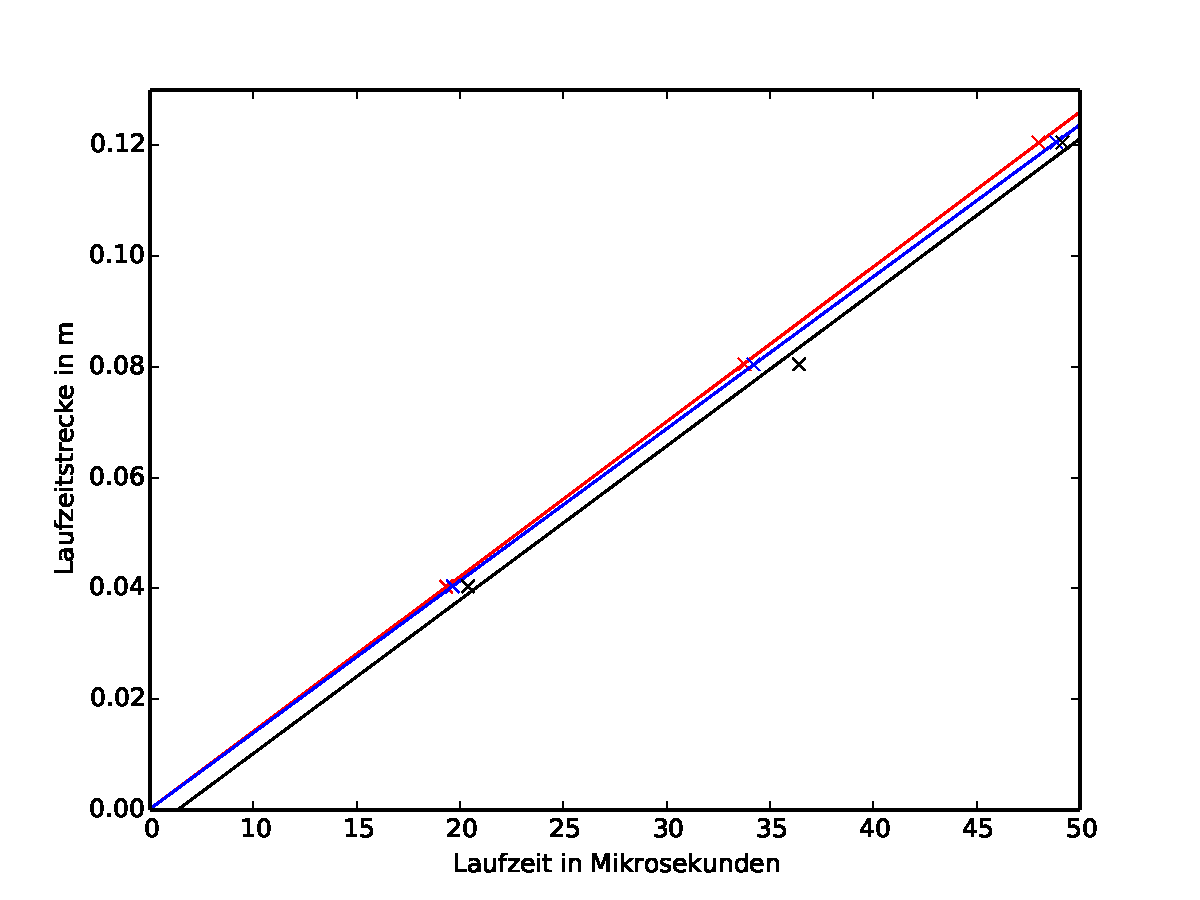
\includegraphics[width=0.9\textwidth]{Bilder/Schallgeschwindigkeit.pdf}
	\caption{Reichweite des Schallimpulses in Abhängigkeit von der Laufzeit, Regression zur Bestimmung der Geschwindigkeit.}
	\label{fig:geschwindigkeit}
\end{figure}

Jeweilige lineare Regression einer Frequenz ergeben die Steigung $m$ und den 
y-Achsenabschnitt $b$, aus denen im Weiteren die Nullstelle $x_0=-\sfrac{b}{m}$ berechnet werden kann.
Die Regressionsparameter und Nullstellen sind in nachfolgender Tabelle \ref{tab:params} angegeben.
\begin{table}[h]
	\centering
	\begin{tabular}{cS[table-format=4.0]S[table-format=-1.1]S[table-format=-1.1]}%S[table-format=4.0\pm3.0] S[table-format=-1.1\pm1.1] S}
	\toprule
	{Plot}&{Steigung $m$/$(\si{\meter\per\second})$}&{y-Abschnitt $b$/$\si{\milli\meter}$}&{Nullstelle $x_0$/$\si{\second}$}\\
	\midrule
		1&\SI{2797(11)}{}&	\SI{0.2(4)e-3}{}& 	\SI{-0.7(13)e-07}{}\\
		2&\SI{2745(6)}{}&	\SI{0.2(2)e-3}{}& 	\SI{-7(7)e-08}{}\\
		3&\SI{2776(181)}{}&	\SI{-4(6)e-3}{}&	\SI{1.3(21)e-06}{}\\
	\bottomrule
	\end{tabular}
	\caption{Regressionsparameter zur Bestimmung der Schallgeschwindigkeit}
	\label{tab:params}
\end{table}
Das Diagramm lässt die Identifikation der Steigung als Schallgeschwindigkeit zu.

Im Idealfall durchqueren die Regressionsgeraden den Koordinatenursprung.
Es liegt zwischen der Sonde und der Oberfläche eine Anpassungsschicht, die systematische Fehler in der Laufzeitmessung hervorruft \cite{skript}.
Diese zusätzlich auftretende Zeit wird als positive Verschiebung der Kurve nach rechts erwartet und ist in Abbildung \ref{fig:geschwindigkeit} anhand der Nullstellen erkennbar.
Die Nullstellen der Regressionen (vgl. Tabelle \ref{tab:params}) weisen für die Impuls-Echo-Methode starke Unsicherheit und einen negativen Nominalwert auf.
Die Nullstelle für die Durchschallungsmethode ist durch die hohe Unsicherheit ungeeignet.
%Die Nullstellen der Regression sind daher für die Betrachtung und Bezifferung der systematischen Fehler unbrauchbar.
Der durch die Anpassungsschicht hervorgerufene Fehler kann daher nicht zuverlässig bestimmt werden und wird somit nicht berücksichtigt.

Der Mittelwert der Schallgeschwindigkeit beträgt
\begin{equation}
	c_\text{Schall}=\SI{2770(60)}{\meter\per\second}
	\label{qu:geschwindigkeit}
\end{equation}
und weicht damit gering vom Literaturwert, $c=\SI{2730}{\meter\per\second}$, um $1.46\,\%$ ab.

\subsection{Simulation einer Materialprüfung}
\label{sec:Auswertung2}
Als Anwendung des Ultraschall-Verfahrens wird ein fehlerhafter Acyrlblock untersucht, dessen Abmessungen in Tabelle \ref{tab:Block_Masze} angegeben sind.
Die mittels Schieblehre gemessenen Kenndaten der Fehler sind in Tabelle \ref{tab:block_fehler} aufgetragen, die Anordnung und Nummerierung der Fehler sind in Abbildung \ref{fig:block} zu erkennen.
\begin{table}[p]
	\centering
	\begin{tabular}{S[table-format=2.0] S[table-format=1.3] S[table-format=1.0]}
	\toprule
	\multicolumn{3}{c}{Maße des Acrylblocks}\\
	{Höhe $h/\:\si{\centi\meter}$}&{Breite $b/\:\si{\centi\meter}$}&{Tiefe $t/\:\si{\centi\meter}$}\\
	\midrule
		15 &8.035  &4\\
		15 &8.030  &4\\
		15 &8.030  &4\\
	\bottomrule
	\end{tabular}
	\caption{Abmessungen des Acrylblocks, Skizze in Abschnitt \ref{sec:Durchfuehrung}, Abbildung \ref{fig:block}}
	\label{tab:Block_Masze}
\end{table}
\begin{table}
	\centering
	\sisetup{table-format=1.3}
	\begin{tabular}{S[table-format=2.0] S[table-format=1.2] S S}
		\toprule
		{} &\multicolumn{3}{c}{Maße der Fehler} \\
		{ID} & {$d$/$\:\si{\milli\meter}$} &{$s_\text{oben}$/$\:\si{\milli\meter}$} & {$s_\text{unten}$/$\:\si{\milli\meter}$}\\
		\midrule
			 1&  2.30& 1.910& 5.970\\
			 2&  1.35& 1.745& 6.160\\
			 3&  5.80& 6.120& 1.340\\
			 4&  4.90& 5.370& 2.180\\
			 5&  3.95& 4.630& 3.015\\
			 6&  3.00& 3.880& 3.870\\
			 7&  3.00& 3.075& 4.660\\
			 8&  2.95& 2.270& 5.470\\
			 9&  2.95& 1.480& 6.290\\
			10&  2.95& 0.690& 7.060\\
			11& 10.00& 5.540& 1.510\\
		\bottomrule
	\end{tabular}
	\caption{Durchmesser der Fehler und deren Abstand zur oberen und unteren Kante des Blocks.}
	\label{tab:block_fehler}
\end{table}
Tabelle \ref{tab:fehlerzeiten} zeigt die Laufzeiten des Ultraschalls im Block, aufgetragen sind die Laufzeiten von beidseitiger Messung.
Analog zu Abschnitt \ref{sec:Auswertung1} wird die Hälfte der gegebenen Zeit ausgewertet.
\begin{table}
	\centering
	\sisetup{table-format=2.2}
	\begin{tabular}{S[table-format=2.0] S S}
		\toprule
		{} &\multicolumn{2}{c}{Laufzeiten} \\
		{ID} &{$t_\text{oben}$/$\:\si{\milli\second}$} & {$t_\text{unten}$/$\:\si{\milli\second}$}\\
		\midrule
			 1& 12.96& 42.26\\
			 2& 11.49& 43.94\\
			 3& 43.42&  8.64\\
			 4& 37.62& 15.60\\
			 5& 32.88& 21.29\\
			 6& 26.77& 27.61\\
			 7& 21.80& 32.88\\
			 8& 15.07& 28.89\\
			 9&  8.90& 44.36\\
			10&  4.00& 50.69\\
			11& 39.31&  9.80\\
		\bottomrule
	\end{tabular}
	\caption{Laufzeit des Schallimpulses bei Ausmessung einer Fehlerstelle ausgehend von oberer und unterer Kante des Blocks.}
	\label{tab:fehlerzeiten}
\end{table}
Mithilfe der in Abschnitt \ref{sec:Auswertung1}, Gleichung \eqref{qu:geschwindigkeit} gefundenen Schallgeschwindigkeit kann die Position der Fehlerstellen über die Laufzeitmessung bestimmt werden. 
Die Ergebnisse sowie deren prozentuale Abweichung sind Tabelle \ref{tab:block_messung} entnehmbar.
\begin{table}
	\centering
	\sisetup{table-format=1.2}
	\begin{tabular}{cSS[table-format=-2.1]SS[table-format=-2.1]SS[table-format=3.1]}
		\toprule
		{} &\multicolumn{2}{c}{Abstand von oberer Kante}&\multicolumn{2}{c}{Abstand von unterer Kante}&\multicolumn{2}{c}{Durchmesser} \\
		{ID}&{$a_\text{oben}$/$\:\si{\centi\meter}$} & {$\mathup{\Delta a_\text{oben}}$/$\:\%$} &{$a_\text{unten}$/$\:\si{\centi\meter}$} & {$\mathup{\Delta a_\text{unten}}$/$\:\%$}&{$d$/$\:\si{\centi\meter}$} & {$\mathup{\Delta d}$/$\:\%$}\\
		\midrule
			1&\SI{1.80(4)}{}&\SI{-5.9}{}	&\SI{5.9(1)}{}&\SI{-1.9}{}		&\SI{4.06(9)}{}&\SI{77}{}\\
			2&\SI{1.59(4)}{}&\SI{-8.7}{}	&\SI{6.1(1)}{}&\SI{-1.1}{}		&\SI{4.5(1)}{}&\SI{233}{}\\
			3&\SI{6.0(1)}{}&\SI{-1.6}{}		&\SI{1.20(3)}{}&\SI{-10.6}{}	&\SI{4.8(1)}{}&\SI{183.1}{}\\
			4&\SI{5.2(1)}{}&\SI{-2.9}{}		&\SI{2.16(5)}{}&\SI{-0.8}{}		&\SI{3.05(7)}{}&\SI{162.3}{}\\
			5&\SI{4.6(1)}{}&\SI{-1.6}{}		&\SI{2.95(6)}{}&\SI{-2.1}{}		&\SI{1.61(4)}{}&\SI{140.7}{}\\
			6&\SI{3.71(8)}{}&\SI{-4.4}{}	&\SI{3.83(8)}{}&\SI{-1.1}{}		&\SI{0.116(3)}{}&\SI{96.12}{}\\
			7&\SI{3.02(7)}{}&\SI{-1.7}{}	&\SI{4.6(1)}{}&\SI{-2.2}{}		&\SI{1.54(3)}{}&\SI{48.8}{}\\
			8&\SI{2.09(5)}{}&\SI{-8.0}{}	&\SI{4.00(9)}{}&\SI{-26.8}{}	&\SI{1.92(4)}{}&\SI{35.1}{}\\
			9&\SI{1.23(3)}{}&\SI{-16.6}{}	&\SI{6.2(1)}{}&\SI{-2.2}{}		&\SI{4.9(1)}{}&\SI{67}{}\\
			10&\SI{0.56(1)}{}&\SI{-19.6}{}	&\SI{7.0(2)}{}&\SI{-0.5}{}		&\SI{6.5(1)}{}&\SI{119}{}\\
			11&\SI{5.5(1)}{}&\SI{-1.6}{}	&\SI{1.36(3)}{}&\SI{-10.0}{}	&\SI{4.09(9)}{}&\SI{140.9}{}\\
			%1&\SI{1.80(4)}{}&\SI{-5.9(21)}{}&\SI{5.86(13)}{}&\SI{-1.9(21)}{}&\SI{4.06(9)}{}&\SI{77(4)}{}\\
			%2&\SI{1.593(35)}{}&\SI{-8.7(20)}{}&\SI{6.09(13)}{}&\SI{-1.1(22)}{}&\SI{4.50(10)}{}&\SI{233(7)}{}\\
			%3&\SI{6.02(13)}{}&\SI{-1.6(21)}{}&\SI{1.198(26)}{}&\SI{-10.6(19)}{}&\SI{4.82(11)}{}&\SI{183.1(18)}{}\\
			%4&\SI{5.22(11)}{}&\SI{-2.9(21)}{}&\SI{2.16(5)}{}&\SI{-0.8(22)}{}&\SI{3.05(7)}{}&\SI{162.3(14)}{}\\
			%5&\SI{4.56(10)}{}&\SI{-1.6(21)}{}&\SI{2.95(6)}{}&\SI{-2.1(21)}{}&\SI{1.607(35)}{}&\SI{140.7(9)}{}\\
			%6&\SI{3.71(8)}{}&\SI{-4.4(21)}{}&\SI{3.83(8)}{}&\SI{-1.1(22)}{}&\SI{0.1164(25)}{}&\SI{96.12(8)}{}\\
			%7&\SI{3.02(7)}{}&\SI{-1.7(21)}{}&\SI{4.56(10)}{}&\SI{-2.2(21)}{}&\SI{1.536(34)}{}&\SI{48.8(11)}{}\\
			%8&\SI{2.09(5)}{}&\SI{-8.0(20)}{}&\SI{4.00(9)}{}&\SI{-26.8(16)}{}&\SI{1.92(4)}{}&\SI{35.1(14)}{}\\
			%9&\SI{1.234(27)}{}&\SI{-16.6(18)}{}&\SI{6.15(13)}{}&\SI{-2.2(21)}{}&\SI{4.92(11)}{}&\SI{67(4)}{}\\
			%10&\SI{0.555(12)}{}&\SI{-19.6(18)}{}&\SI{7.03(15)}{}&\SI{-0.5(22)}{}&\SI{6.47(14)}{}&\SI{119(5)}{}\\
			%11&\SI{5.45(12)}{}&\SI{-1.6(21)}{}&\SI{1.359(30)}{}&\SI{-10.0(20)}{}&\SI{4.09(9)}{}&\SI{140.9(9)}{}\\
		\bottomrule
	\end{tabular}
	\caption{Über die Schalllaufzeit gemessene Abstände und Maße der Fehlerstellen und deren Abweichungen von der Messung per Schieblehre.}
	\label{tab:block_messung}
\end{table}

Abbildungen \ref{fig:b_scan_4} und \ref{fig:b_scan_2} zeigen die B-Scans des fehlerbehafteten Blocks.
Erkennbar ist, dass eine Erhöhung der gewählten Frequenz $f$ in einer höheren Auflösung resultieren, die allerdings eine geringere Intensität zeigen.
Es ist daher zweckmäßig, eine größtmögliche Frequenz zu wählen, bei welcher die Störstellen eindeutig zu erkennen sind.
\begin{figure}[hp]
	\centering
	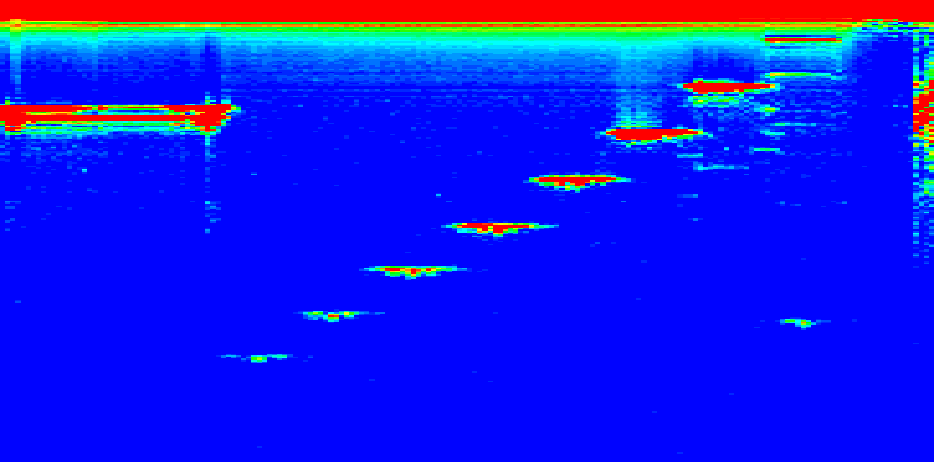
\includegraphics[width=0.85\textwidth]{Bilder/Block_4Mhz.png}
	\caption{B-Scan des fehlerhaften Blocks bei der Frequenz $f=\SI{4}{\mega\hertz}$}
	\label{fig:b_scan_4}
\end{figure}
\begin{figure}[hp]
	\centering
	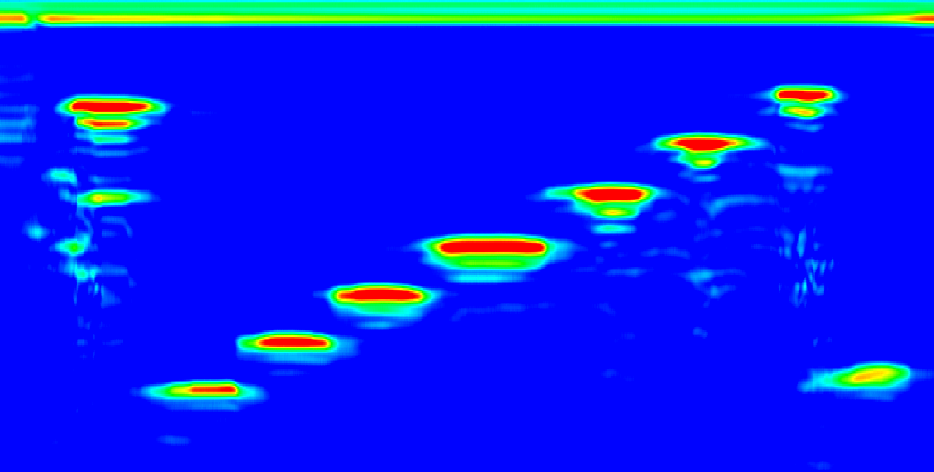
\includegraphics[width=0.85\textwidth]{Bilder/Bscan_2.png}
	\caption{B-Scan des fehlerhaften Blocks bei der Frequenz $f=\SI{2}{\mega\hertz}$}
	\label{fig:b_scan_2}
\end{figure}
\newpage
\subsection{Messung an einem Modell des menschlichen Auges}
\label{sec:Auswertung3}
Die in vorangegangenen Kapiteln gewonnenen Erkenntnisse über Ultraschall in Materie \ref{sec:Auswertung1} und deren anwendungsbezogener Nutzen, etwa in Medizin, \ref{sec:Auswertung2}. wird anhand einer  Messung an einem Modell des menschlichen Auges simuliert.
\begin{figure}[h]
	\centering
	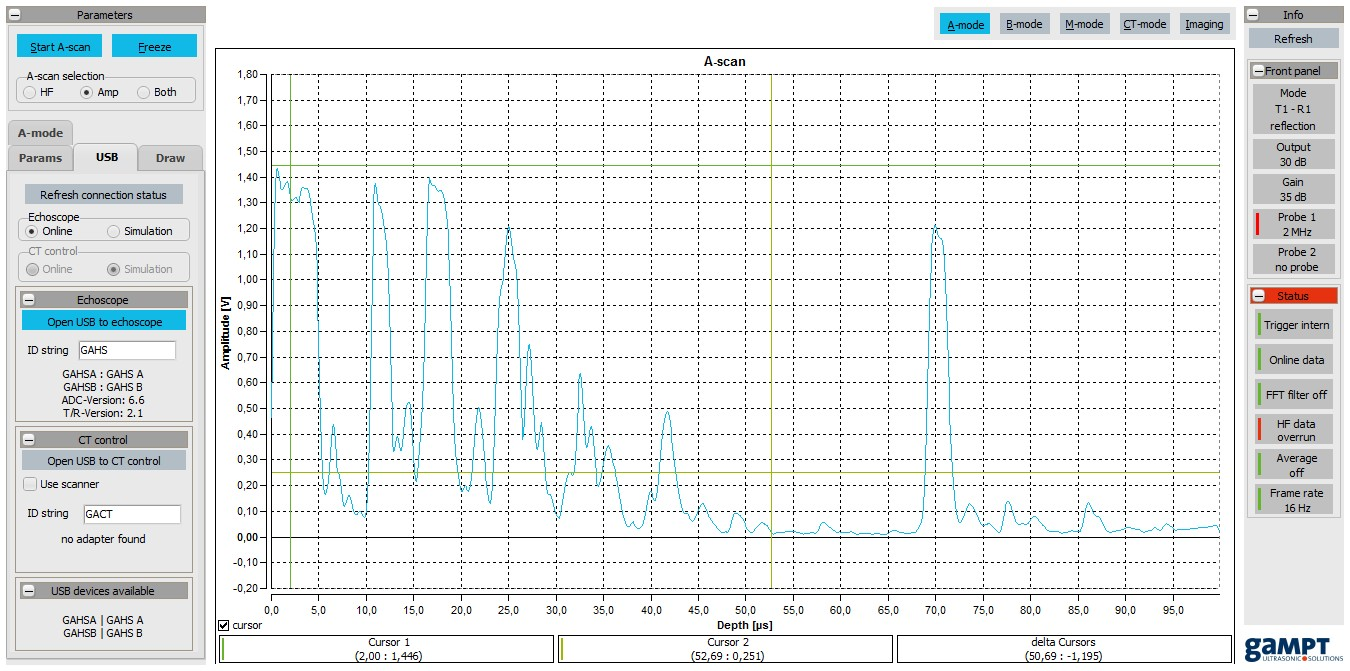
\includegraphics[width=0.9\textwidth]{Bilder/Auge.jpg}
	\caption{A-Scan des Augenmodells.}
	\label{fig:eye_scan}
\end{figure}
Abbildung \ref{fig:eye_scan} zeigt den A-Scan eines vorliegenden Augenmodells.
Die geringe Anzahl der deutlich separierbaren Maxima erlaubt deren Zuweisung auf die Bestandteile des Auges, an denen der Schall reflektiert worden sein könnte. 
Das Maximum in Umgebung von $\SI{2}{\micro\second}$ ist ein Reflexionsmaximum, die darauffolgenden Maxima mit einer Mindestamplitude von $\SI{1}{\volt}$ sind Hornhaut, Vorder- und Rückseite der Linse und der Retina zuzuordnen.

Mit den relativen Zeitabständen zwischen den Maxima ergeben sich Abstände im Auge, die in Tabelle \ref{tab:auge} zu entnehmen sind.
Die Schallgeschwindigkeiten sind dabei den Materialien angepasst; es gilt $c_\text{L} = \SI{2500}{\meter\per\second}$ in der Linse sowie $c_\text{GK} = \SI{1410}{\meter\per\second}$ im Glaskörper.
Da das Modell im Maßstab 1:3 das menschliche Auge darstellt, kann auf die realen Werte umgerechnet werden.
\begin{table}[h]
	\centering
	\begin{tabular}{cccc}
	\toprule
	\multicolumn{4}{c}{Abstände}\\
	{Objekte}&{Zeit $t/\:\si{\micro\second}$}&{in Modell $a_0/\:\si{\centi\meter}$}&{im Auge $a_1/\:\si{\centi\meter}$}\\
	\midrule
		{Hornhaut-Linse}&{5.5}&{1.5}&{0.5}\\
		{Linse}&{8}&{1.9}&{0.6}\\
		{Linse-Retina}&{45}&{6.3}&{2.1}\\
		%{}&\multicomlumn{3}{c}{Abstände im Augenmodell}
		%{}&{Hornhaut-Linse $a_\text{HL}/\:\si{\centi\meter}$}&{Linsendicke $a_\text{L}/\:\si{\centi\meter}$}&{Linse-Retina $a_\text{LR}/\:\si{\centi\meter}$}\\
		%1.109(24)&0.693(15)&1.109(24)&6.24(14)
	\bottomrule
	\end{tabular}
	\caption{Abstände im Augen-Modell}
	\label{tab:auge}
\end{table}

Die Linsendicke, $d_\text{Linse}=\SI{0.6}{\centi\meter}$, weicht von der Literaturangabe, etwa $\SI{0.4}{\centi\meter}$, um $50\%$ ab.
Der Augendurchmesser, $d_\text{Auge}=\SI{3.1}{\centi\meter}$, weicht von der Literaturangabe, etwa $\SI{1.7}{\centi\meter}$ bis $\SI{2.4}{\centi\meter}$, vergleichbar stark ab \cite{medizinmann}.
Beide Messungen geben damit nicht mehr als die Größenordnung zuverlässig an.